% !TEX root = Eco-Model.tex
\section{Background} % (fold)
\label{sec:background}

As an application of networked manufacturing, cloud manufacturing proposed by ...

(problems background to form the ecosystem)

\subsection{List of basic terminology} % (fold)
\label{sub:list_of_basic_terminology}
here we goes the terminology that will use in the following subsections within this section. all the related basic terms will in italics fonts.
\begin{itemize}
	\item order
	\item task correspond to capacity
	\item resource
	\item capacity is the function of a resource. like quantity
	\item service is the bundle of capacities. the proportion of the capacities.
	\item 
\end{itemize}
% subsection list_of_basic_terminology (end)

\subsection{Cloud manufacturing} % (fold)
\label{sub:cloud_manufacturing}

\subsubsection{Cloud manufacturing architecture}
\label{subs:cloud manufacturing architecture}
Combined with the background of the research problem and other scholars' previous study in cloud manufacturing, we proposed an improved framework that suits for cloud manufacturing environment as shown in \autoref{fig:structure}.
\begin{figure}[htbp]
\centering
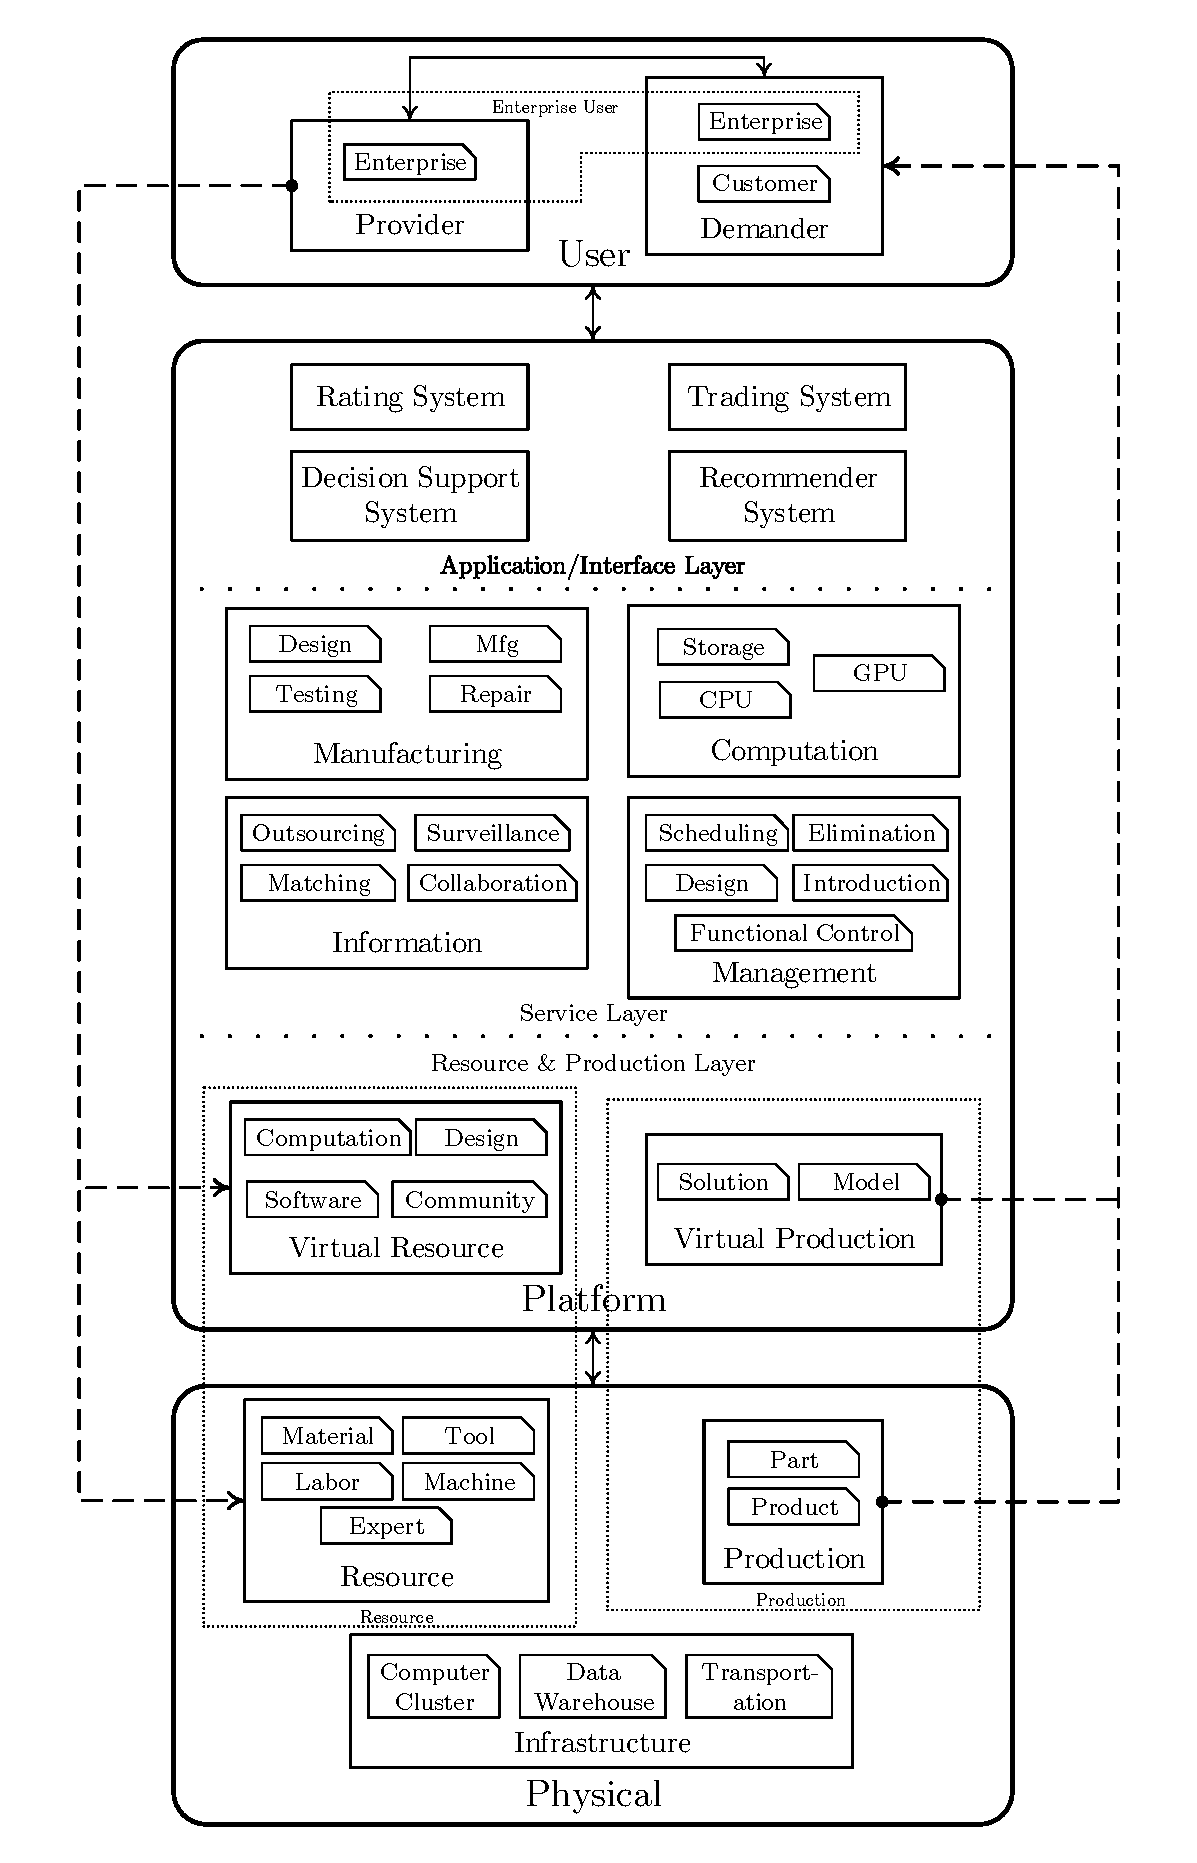
\includegraphics[scale = .3, trim = 0 15 0 35]{Cloud_Mfg_Structure.pdf}
\caption{Cloud manufacturing architecture with main flows}
\label{fig:structure}
\end{figure}

The architecture of cloud manufacturing is mainly composed of three parts, namely, \begin{inparaenum}[1)]
\item user,
\item platform and
\item physical base
\end{inparaenum}, that are connected by material or information flows. A simple version of conception for cloud manufacturing architecture we study here can be described as follows:
\begin{compactdesc}
\item [User] part describes the generalized role who takes part in the trading activities in the cloud manufacturing system, basic role of user are manufacturing service provider and manufacturing service demander, whom can be called as \textit{provider} and \textit{demander} for short respectively, from the functional point of view. Meanwhile, these part can also be classified into enterprise user and customer, from the practical point of view. In addition, it's possible for user to act as both demander and provider simultaneously if administrator give the authority to the user, so we can categorize the user in 3 basic types as described in \autoref{fig:usertype} and \autoref{tab:usertype}. Both functional and practical are important perspective for later analysis in following sections.
\item [Platform] is operating with the control of administrator and this part consists of 3 main layers namely
	\begin{inparaenum}[1)]
	\item application/interface layer,
	\item service layer and
	\item resource \& production layer
	\end{inparaenum}.
Service is the core concept in cloud manufacturing, so service layer is the core in the cloud manufacturing platform. With the help of related technology in servitization, manufacturing resource and production can be encapsulated into services, then these services can be acquired by users with the well designed applications or interfaces.
\item [Physical Base] part includes the basic infrastructure, resource and production. It's worth mentioning that part of resources and production can even be virtualized with some services the platform provides.
\end{compactdesc}


\begin{figure}[htbp]
	\centering
	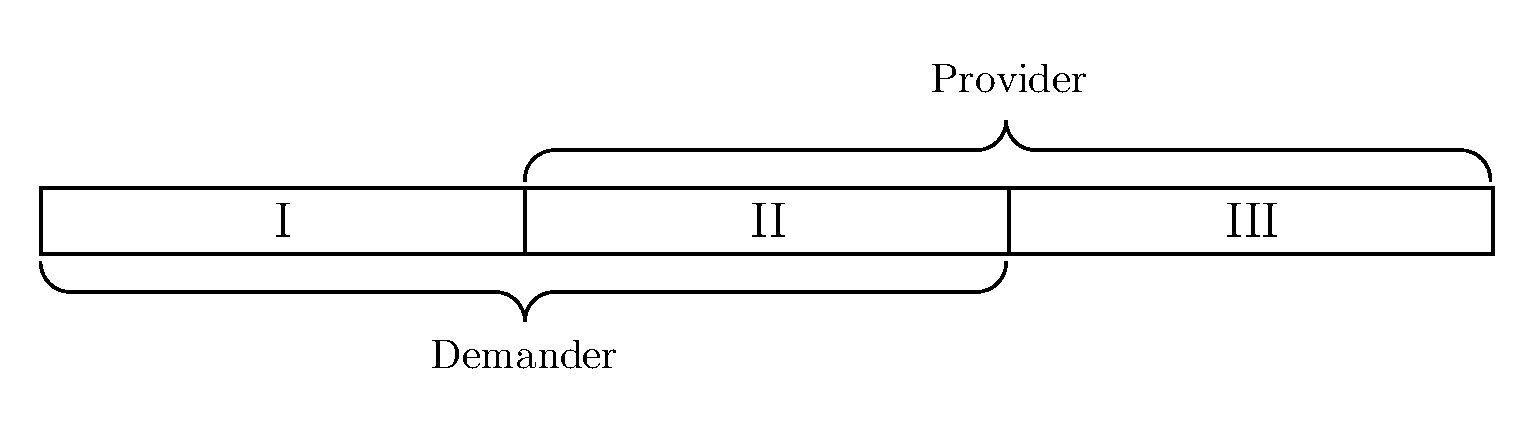
\includegraphics[width=.7\textwidth]{usertype.pdf}
	\caption{Simple explanation of user type}
	\label{fig:usertype}
\end{figure}

\begin{table}[htbp]
	\caption{Simple explanation of user type}
	\label{tab:usertype}
	\centering
	\tiny
	\begin{tabularx}{\textwidth}{llX}
	\toprule
	\textbf{Type} & \textbf{Name} &  \textbf{Concise Description}\\
	\midrule
	I			& Pure demander &  Submit manufacturing tasks and make evaluation of provider.\\
	II 			& Complex user 	&  Usually a pure provider submit part of its task, it becomes the complex user and changes the operation model of the user.\\
	III 		& Pure provider &  Provide manufacturing services and makes evaluation demander.\\
	\bottomrule
	\end{tabularx}
\end{table}
% Before the emendation of the roles, some related standard name should be taken:

As defined above, Enterprise User is the special case of the User(short for Generalized User) that purely provides manufacturing services and the Customer User is similarly defined.

Hence, there is only two roles in the Ecosystem worth to be studied: User and Administrator, the proportion of user type could be adjusted as the runtime of the system goes by.

\begin{figure}[htbp]
\centering
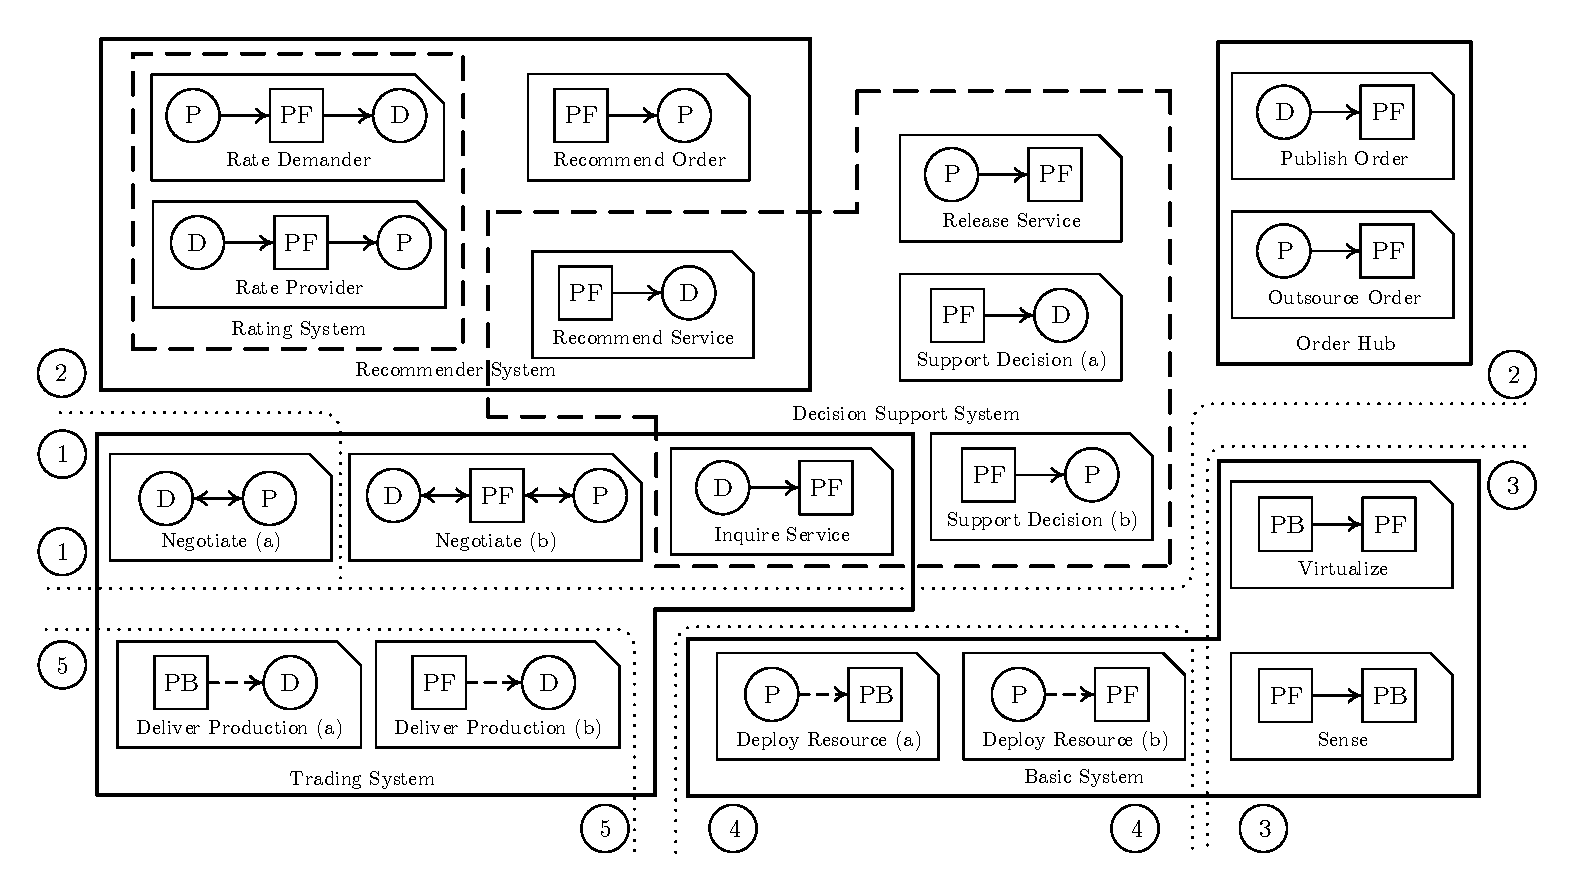
\includegraphics[scale = .3, trim = 0 15 0 10]{supplementary.pdf}
\caption{Supplementary illustration for \autoref{fig:structure}}
\label{fig:supplementary}
\end{figure}

With the supplementary illustration of \autoref{fig:supplementary}, which categorizes the main applications in cloud manufacturing environment with the fore-mentioned flows that marked by circled number (i.e. \textcircled{\small{1}}) and corresponding to the same symbol in \autoref{fig:structure}, we can simply describe the main activities within the cloud manufacturing system. In \autoref{fig:supplementary}, we denote provider, demander, platform and physical base as \textbf{P}, \textbf{D}, \textbf{PF} and \textbf{PB} respectively. The overlap among application districts implies the complexity of the system, so that we will analyze these applications coordinately from a systematic view.

\subsubsection{Operation model of platform}
\label{ssub:operation_model_of_platform}
Platform carries most of the activities illustrated in \autoref{fig:supplementary}, so it's important to design an operation model for administrator to manage these activities. This model enables modules that appeared in xxx such as \textit{service packager}, \textit{task decomposer} , \textit{service search engine}, etc., but we only study the modules in for they're the core in the evolutionary process in this paper.

\begin{table}[tb]
	\caption{Core modules in operation model of platform}
	\label{tab:core_module_in_platform}
	\centering
	\scriptsize
	\begin{tabularx}{\textwidth}{llX}
	\toprule

	\textbf{Module} & \multicolumn{2}{l}{\textbf{Function with concise description}}  \\
	\midrule
	\multirow{2}*{Population controller}		& Adder: 		& To introduce resource provider into the system\\
												& Subtracter: 	& To eliminate resource provider from the system\\
	\hline
	\multirow{2}*{Authority tuner}				& Raiser:	& Raise the authority value of the provider \\
												& Reducer: & Reduce the authority value of the provider\\
	\hline
	\multirow{3}*{Recommender}					& Matcher: & Match task with a bunch of alternative services \\
												& Adjuster: & Change provider's rank based on history\\
												& Promoter: & To promote fresh resource provider \\
	\bottomrule
	\end{tabularx}
\end{table}

platform model is about the part of decision making	agent of platform.

\subsubsection{Operation model of users}
\label{subs:Operation model of users}
The \textit{demander} mentioned in \autoref{subs:cloud manufacturing architecture} publishes its demand as order that can be decomposed into tasks by \textit{task decomposer} module in platform, while the \textit{provider} mentioned in \autoref{subs:cloud manufacturing architecture} publishes its resource as capacity that can be packaged into services by \textit{service packager} module in Platform. In order to do more accurate study on users, we classified users into 3 basic types as shown in \autoref{fig:usertype}. With concise explanation in \autoref{tab:usertype}, we can illustrate the operation model in \autoref{fig:useroperation}.

\begin{figure}[htbp]
\centering
\subfloat[Pure demander]{
\includegraphics[width=0.75\textwidth]{demander_main_process}\label{fig:demanderprocess}}\\
\subfloat[Complex user]{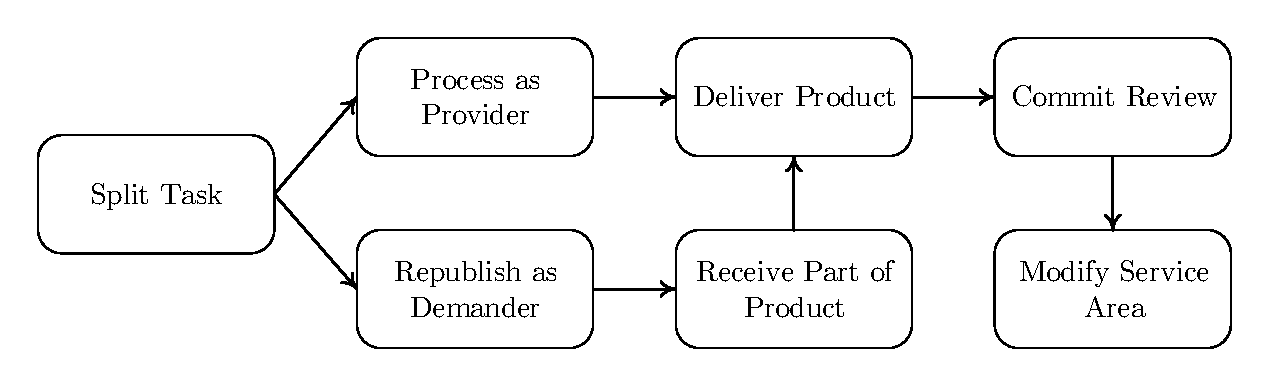
\includegraphics[width=0.75\textwidth]{complex_main_process}\label{fig:complexprocess}}\\
\subfloat[Pure Provider]{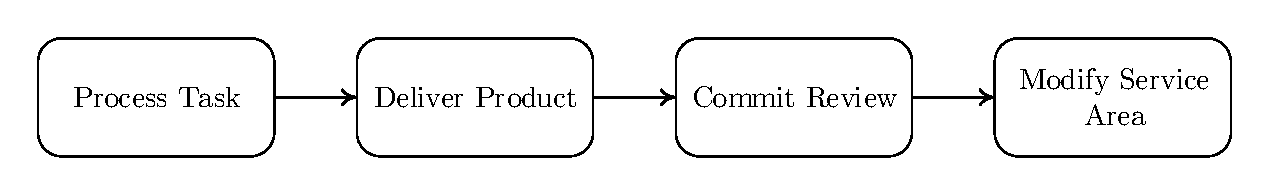
\includegraphics[width=0.75\textwidth]{provider_main_process}\label{fig:providerprocess}}
\caption{Main operational processes}
\label{fig:useroperation}
\end{figure}

The main operational process of pure demander(\autoref{fig:demanderprocess}) starts with its decomposed task. Then, with the help of \textit{recommender} module, pure demander search and select appropriate service, trade with the one or multi service provider according to the \textit{task decomposer}, receive the product delivered by the provider at due date and commit the review of the product. The committed review will affect the authority value of the provider, that good review raise the value and vise versa.

The main operational process of pure provider(\autoref{fig:providerprocess}) starts with a task call, then pure provider process the task with its resource. After the accomplishment of the task, pure provider deliver products to demander from the call. It will also commit the review of the demander and make a modification of its service area. By the way, this modification of provider's service area play key role in the evolution of user we will discuss in \autoref{ssub:microscopic_evolution}.  

The main operational process of complex user(\autoref{fig:complexprocess}) combines the two above process with additional decision step. This decision split the task into two parts, that one of them will be processed by itself as a provider user and the other one will be processed by other provider as if the complex user act as a demander. This operational process relies heavily on the service area of the complex user, so the modification of service area is the key to the study.

user's model is the part of decision making agent of users.



\subsection{The evolution of manufacturing ecosystem} % (fold)
\label{sub:the_evolution_of_manufacturing_ecosystem}
Before the realization of the operation model mentioned above(\autoref{subs:Operation model of users}), we will analyze the evolution path in both micro and macro view of manufacturing ecosystem w.r.t. the domain in cloud manufacturing. The overall evolution process is illustrated in \autoref{fig:overallevolution},
\begin{figure}[htbp]
	\centering
	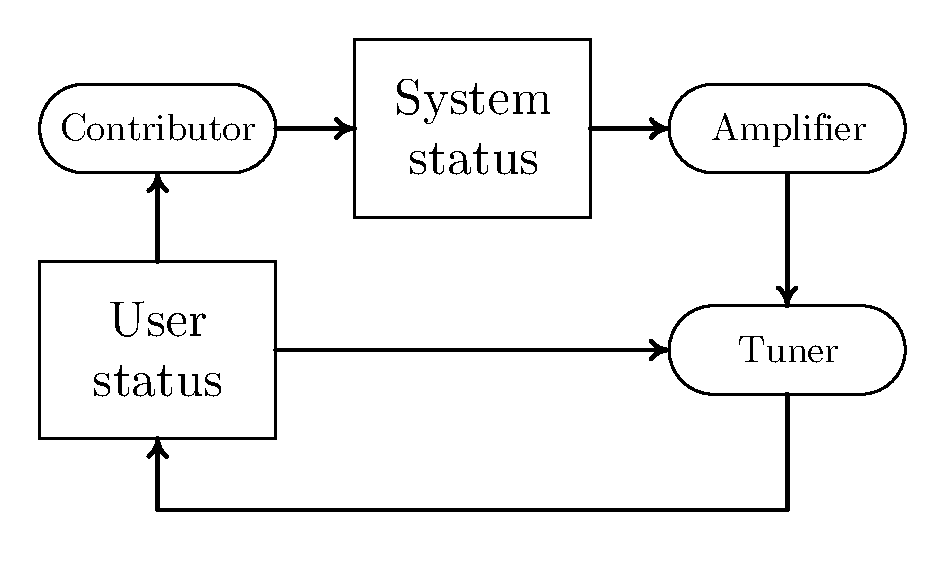
\includegraphics[width=.5\textwidth]{evolutionview}
	\caption{Overall evolution process}
	\label{fig:overallevolution}
\end{figure}
the microscopic evolution corresponds to the change of user status while the macroscopic evolution corresponds to the change of the system status.

\subsubsection{Microscopic evolution} % (fold)
\label{ssub:microscopic_evolution}

by both type of agents, more on user agent, the platform agent will change a individual by affect the individual's decision, not directly means.

User is the basic activity individual in the manufacturing ecosystem, and their \begin{inparaenum}[1)]
\item type,
\item status and 
\item niche width
\end{inparaenum} will be changed by the decision they've made. 
All these changes contribute to microscopic evolution of the ecosystem. More specifically, type change describes the change of user's type among pure demander, pure provider and complex user; status change describes weather a user in the ecosystem or not; niche width change describes the importance or condition of the user, especially the provider and we will only discuss the provider's niche width in this paper. \autoref{tab:userchange} concludes the appearances that we will study in this paper.

\begin{table}[htbp]
	\caption{Users' changes}
	\label{tab:userchange}
	\centering
	\scriptsize
	\begin{tabularx}{\textwidth}{llX}
	\toprule
	\textbf{Change} & \multicolumn{2}{l}{\textbf{Appearance with concise description}}\\
	\midrule
	\multirow{3}*{Type}			& Complex user $\to$ Pure demander: & User stop provide its resource\\
								& Complex user $\to$ Pure provider: & User shrink service area that only contains its own service \\
								& Pure provider $\to$ Complex user: & User extend service area that starts to contain service from others' \\
	\midrule
	\multirow{4}*{Status} 		& Pure demander enter ecosystem: &	One pure demander starts to publish orders\\
								& Pure demander exit ecosystem: & One pure demander be banned to publish orders\\
								& Pure provider enter ecosystem: & Administrator introduces one provider into the ecosystem\\
								& Pure provider exit ecosystem: & Administrator eliminates one provider form the ecosystem\\
	\midrule
	\multirow{2}*{Niche width} 	& Widen: & One provider extends its service area\\
								& Narrow down:  & One provider shrinks its service area\\
	\bottomrule
	\end{tabularx}
\end{table}



% subsubsection microscopic_evolution (end)

\subsubsection{Macroscopic evolution} % (fold)
\label{ssub:macroscopic_evolution}
Comes form both of the agents. more on platform agent.
indirect: the group effect.

Individual evolution will lead to the evolution of the whole ecosystem and the overall effect is greater than the sum of these individuals.

the amount, diversity, operation pattern recognition and service cycle rate are the topics of macroscopic evolution.

\begin{table}[htbp]
 	\caption{Macroscopic evolution}
 	\label{tab:macroevolution}
 	\centering
 	\scriptsize
 	\begin{tabularx}{\textwidth}{llX}
 	\toprule
 	\textbf{column 1} & \multicolumn{2}{l}{\textbf{Appearance with concise description}} \\
 	\midrule
 	Amount & & \\
 	Diversity & & \\
 	Service cycle rate & & \\
 	\bottomrule
 	\end{tabularx}
 \end{table} 


% subsubsection macroscopic_evolution (end)

\subsection{Main topics and their academic importance}
% 提一下云制造生态环境中的应用、模块,主要强调这些模块之间的交互,会产生怎样的作用。 目前云制造缺乏相关运作式的讨论,而商业模式中的不同行为会影响、改变、涌现。
As shown in \autoref{fig:structure},

the core is about the decision making all the time, individuals' decision making will affect themselves directly, that will lead to most of the microscopic evolution, and the group effective will contribute part of the macroscopic evolution 

Rating system, decision support system, recommender system,
detail info will seen in
Modular approaches are widely used to decompose a complex system into smaller subsystems according to their functions. For example, Yang and Li (2011) divided a cloud manufacturing services management and control platform into seven functional modules such as system management module, production management module and so on

so, the topic here is the design of both decision making agents.
% subsection the_evolution_of_manufacturing_ecosystem (end)
% section background (end)
